%%%%%%%%%%%%%%%%%%%% author.tex %%%%%%%%%%%%%%%%%%%%%%%%%%%%%%%%%%%
%
% sample root file for your "contribution" to a proceedings volume
%
% Use this file as a template for your own input.
%
%%%%%%%%%%%%%%%% Springer %%%%%%%%%%%%%%%%%%%%%%%%%%%%%%%%%%


\documentclass{svproc}
%
% RECOMMENDED %%%%%%%%%%%%%%%%%%%%%%%%%%%%%%%%%%%%%%%%%%%%%%%%%%%
%

% to typeset URLs, URIs, and DOIs
\usepackage{url}
\usepackage{graphicx}
\def\UrlFont{\rmfamily}
\usepackage{amsmath}
\usepackage{amssymb}
\usepackage[ruled,vlined, linesnumbered]{algorithm2e}
\usepackage{algorithmic}

\begin{document}
\mainmatter              % start of a contribution
%
\title{PyChrono and gym-chrono: a Deep Reinforcement Learning framework leveraging Multibody Dynamics to \\ control Autonomous Vehicles and Robots.}
%
\titlerunning{PyChrono and gym-chrono}  % abbreviated title (for running head)
%                                     also used for the TOC unless
%                                     \toctitle is used
%
\author{Simone Benatti\inst{1} \and Aaron Young\inst{2} \and
Asher Elmquist \inst{2} \and Jay Taves \inst{2} \and Radu Serban \inst{2} \and
Dario Mangoni\inst{1} \and Alessandro Tasora\inst{1} \and
Dan Negrut \inst{2} }

%
\authorrunning{Simone Benatti et al.} % abbreviated author list (for running head)
%
%%%% list of authors for the TOC (use if author list has to be modified)
%\tocauthor{Ivar Ekeland, Roger Temam, Jeffrey Dean, David Grove,
%Craig Chambers, Kim B. Bruce, and Elisa Bertino}
%
\institute{Dipartimento di Ingegneria ed Architettura, University of Parma, Parma, Italy,\\
\email{simone.benatti@studenti.unipr.it}
\and
University of Wisconsin -- Madison, Madison, WI, USA}

\maketitle              % typeset the title of the contribution

\begin{abstract}
gym-chrono is a set of simulated environments for Deep Reinforcement Learning (DRL) extending OpenAI Gym \cite{Brockman16Gym} with robotics and autonomous driving tasks. The physics of these environments is simulated thanks to Project Chrono~\cite{chronoOverview2016}, an open-source multi physics simulation engine capable of simulating Multibody Dynamics with constraints and smooth or non-smooth contacts. The most used Deep Learning frameworks (such as PyTorch and Tensorflow ) have Python API, thus using Python to implement DRL algorithms is the most convenient option. For this reason a condition for the creation of these environments has been the development of PyChrono, a Python module consisting of the Python bindings to Project Chrono C++ API, to effectively interface the simulation capabilities of Project Chrono with Deep Learning frameworks.
\keywords{Multi-Body, Simulation, Deep Learning}
\end{abstract}
%




%%%%%%%%%%%%%%%%%%%%%%%%%%%%%%%%%%%%%%%%%%%%%%%%%%%%%%%%%%%%


\section{Introduction}

%containing also the motivation and the purpose of the study together with a brief summary of previous works on the topic
Reinforcement Learning (RL) \cite{SuttonBarto1998RL}  is a Machine Learning technique based on agent-environment interactions: at each interaction the agent performs an \textit{action} and collects the \textit{state} of the system and a \textit{reward} measuring its performance in solving some task; the goal of RL is, given the state, picking the action that maximizes the expected sum of reward, thus solving the task. In the last few years \cite{Mnih13} Deep Learning used in conjunction with RL (called Deep Reinforcement Learning, DRL) has demonstrated to be a viable approach to solve complex real-world robotics tasks \cite{openai2018HandManipulation}. DRL methods, like any other Deep Learning approach, require large dataset to optimize the Neural Networks, these dataset can by collected by sampling from real robots or through simulation, the latter being safer, cheaper and easier to set up and parallelize.

The results obtained in DRL-based controls has arisen interest in physics engine providing a Python API. The DRL community heavily relies MuJoCo \cite{todorovMujoco2012} and PyBullet \cite{bulletPhysicsEngine2020}
for robotics environments and on CARLA \cite{carlaAVsim2017} and AirSim \cite{shah2018airsim}for autonomous driving.

We provide in a single Python framework a set of reinforcement learning environments that feature:
\begin{itemize}
    \item Multibody Dynamics simulation with constraints and smooth or non-smooth contacts
    \item Deformable bodies simulation through Finite Element Analysis simulation
    \item Vehicle dynamics simulation tools
    \item Sensor simulation
\end{itemize}

\section{PyChrono}
\subsection{Interpreted Language}
Python is an interpreted language: This brings obvious upsides in terms of ease of use, but greatly limits the computational performance. Python has also limited parallelization capabilities, since each Python process is locked on a single thread (Global Interpreter Lock, also known as GIL).

The reason behind Python success in high performance computing is the interfacing with compiled libraries through \textit{Bindings}. In this scenario Python is used as high level interface.

\subsubsection{SWIG}
To create a Python \textit{Wrapper} for Chrono we rely on SWIG \cite{SWIG96} (Simplified Wrapper and Interface Generator). It generates bindings between C/C++ code and common scripting languages, such as Perl, C\# and Python, without need to modify the underlying code.

What the Python/C++ bindings do is creating hooks to call the compiled libraries, therefore while the functions are called from the Python API, the computation, under the hood, calls the same libraries as the C++ API. By doing this, the computational overhead of using Python is minimal, while getting the usage and compatibility benefits.

Besides allowing to solve the Python performance issues, Python bindings also allow to use multithreading when it is leveraged by the underlying code. This fits well into Python purpose, being an high-level programming language relying on binary libraries for computation.
In figure \ref{fig:OpenMP} we show how PyChrono can still use multiple CPU cores while being used from Python in a simulation with finite elements and contacts. 

\begin{figure}[ht]
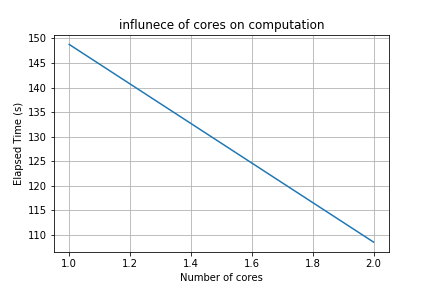
\includegraphics[width=0.75\textwidth]{Figures/OpenMPtest.png}
\caption{Speedup in computation when parallelizing the task on 2 cores.}
\label{fig:OpenMP}
\end{figure}

\subsection{Package Features}
\subsubsection{Multi Body Dynamics}
PyChrono wraps the Multi Body Dynamics simulation classes of Project Chrono, providing:
\begin{itemize}
    \item Multi Body constrained Dynamics
    \item Smooth and non-smooth contacts
    \item FEA based deformable bodies: beams, shells and 3D elements.
    \item Various solvers and timesteppers
    \item 1D shaft systems simulation
\end{itemize}
These features are provided by 3 sub-modules: \textit{core, fea }and \textit{mkl} (the latter only providing the interface to MKL PARDISO solver)
\subsubsection{Modeling and Visualization Tools}
The \textit{irrlicht} and \textit{postprocess} sub-module provide real-time 3D rendering and post processing tools (such as POV-Ray scripts for higher quality rendering).
\subsubsection{Vehicle Dynamics}
Wrapping all of Project Chrono vehicle simulation classes, PyChrono supports template-based tools for modeling wheeled and tracked vehicles. The templates include wheeled vehicle parts (steering, suspension, wheel etc.), tracked vehicle parts (track-shoe, sprocket, idler etc.), terrain, powertrain and driver. 
For some of these classes have several sub-classes that represent different mechanisms or physics detail. To mention a couple, there are 19 different suspension mechanisms (Double Wishbone, Multi Link etc) and 13 different tire models (rigid, Pacejka, deformable etc.). PyChrono vehicle also provides complete vehicle models that combined the aforementioned parts to give the user a pre-cooked vehicle model. This feature is especially welcome in contexts, such as the topic of this work, in which the focus is not on a specific vehicle model, but rather on vehicle dynamics simulation in general.
\subsubsection{Sensor Simulation}
The \textit{sensor} sub-module wraps Chrono::Sensor functionalities, being:
\begin{itemize}
    \item Support for Exteroceptive sensing, which is the sensing providing scene information. More specifically it uses NVIDIA OptiX library ray tracing to simulate camera and Lidar sensors, whose process runs on the GPU.
    \item Support for Interoceptive sensing, which is the sensing providing information from the simulation itself (although processed, such as converting positions to GPS coordinates). This family inludes inertial measurment units sensors (IMU) and GPS.
    \item Parametrization of sensors specifics (update rate, field of view, lag) and noise models for every sensor supported.
\end{itemize}
\paragraph{Sensor Data Pipeline in Python API}
Camera and Lidar sensors outputs (RGB images and point clouds respectively) memory footprint are large and in a vision-based control moving these data at each controller step might be a major bottleneck. To solve this, we cast map the data as NumPy arrays \cite{van2011numpy} using the NumPy SWIG interface. Doing so, the NumPy array class is wrapped around the raw array without instantiating new memory. This comes with no overhead, saving both time and memory.

\subsubsection{Deployment of the Python package}
Anaconda is a Python distribution that creates \textit{virtual environments} of Python to have various version of Python and Python packages on the same machine. It also manages the installation and dependencies management of Python packages through the Conda Package Manager. Through Anaconda toolchain it is possible to create packages using \textit{conda-build} and make it available to the public through the Anaconda Cloud platform.

For these reasons we identified Anaconda packages as the right tool to deploy and distribute PyChrono.
This deployment strategy makes the simulation tool more easily available for the user, and PyChrono had great benefited from this, having reached more than 3000 downloads at the time of writing this document.


\section{gym-chrono}
\subsection{Motivations and Features}
gym-chrono is a Python module that provides a set of Reinforcement Learning virtual environments that use PyChrono for physics simulation. This package is an extension of OpenAI gym package, and all its environment inherit from the OpenAI gyn environment class. Since every third-party algorithms and DRL framework is compatible with OpenAI gym environments, they can be used for gym-chrono environments as well. The same goes for environments utilities, such as the subprocess environments parallelization provided by OpenAI Baselines. Moreover, once the package is installed through Pytohn package manager, its environments can be called from anywhere in the machine by their unique ID.

\subsection{Environments}
This is a list of  the gym-chrono environments. We will refer to state as $s$ and the action as $a$
\subsubsection{Benchmarking Environments}
These 2 environments are the simplest of the set, and are used to benchmark algorithms or hyperparameters tuning, without the pretense of modeling real world robots. The first is a reversed pendulum to be balanced ($s \in \mathbb{R}^4$, $a \in \mathbb{R}$), the second a 4-legged walker called \textit{ant} ($s \in \mathbb{R}^{30}$, $a \in \mathbb{R}^8$)

\begin{figure}[ht]
 \begin{minipage}[b]{0.6\linewidth}
    \centering
    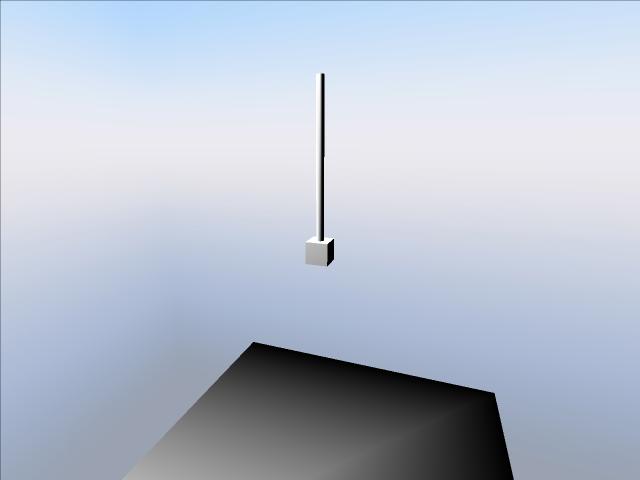
\includegraphics[width=0.75\textwidth]{ProcSci_TeX/Figures/pendulum.png}
    \caption{Pendulum}
    \label{fig:pendulum}
 \end{minipage}
 \hspace{0.4cm}
 \begin{minipage}[b]{0.6\linewidth}
    \centering
    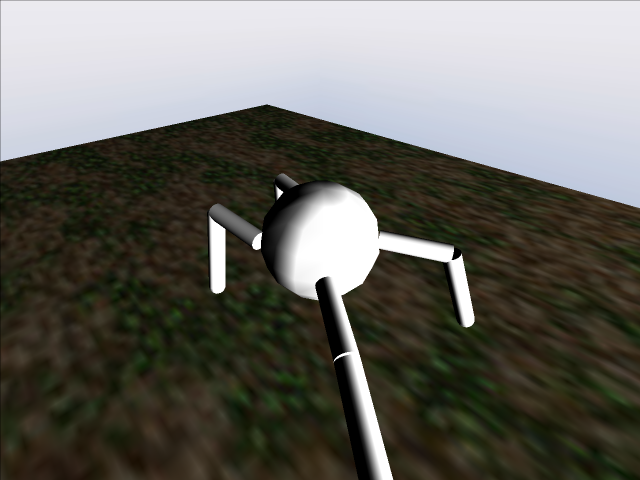
\includegraphics[width=0.75\textwidth]{ProcSci_TeX/Figures/ant.png}
    \caption{Ant}
    \label{fig:ant}
 \end{minipage}
\end{figure}

\subsubsection{Robotics Environments}
These environments feature models of real robots created with our SolidWorks plugin. We provide a 6DOF robitc arm \ref{fig:Comau} that has to reach a random end-effector position without colliding with the floor or its own parts ($s \in \mathbb{R}^{18}$, $a \in \mathbb{R}^6$) and a hexapod \ref{fig:Hexa} that must learn to walk ($s \in \mathbb{R}^{53}$, $a \in \mathbb{R}^{18}$).

\begin{figure}[ht]
 \begin{minipage}[b]{0.6\linewidth}
    \centering
    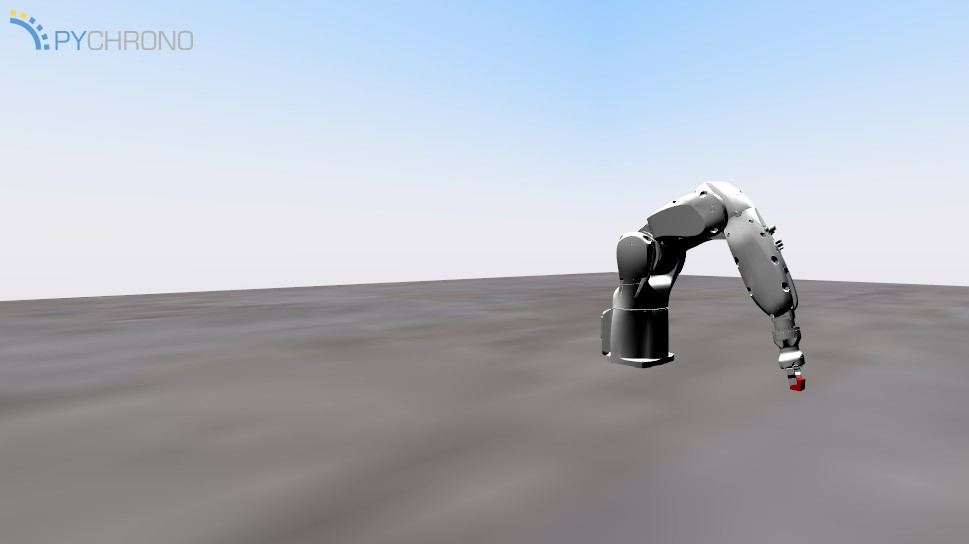
\includegraphics[width=0.75\textwidth]{ProcSci_TeX/Figures/Comau.jpg}
    \caption{Robotic Arm Environment}
    \label{fig:Comau}
 \end{minipage}
 %\hspace{0.4cm}
 \begin{minipage}[b]{0.6\linewidth}
    \centering
    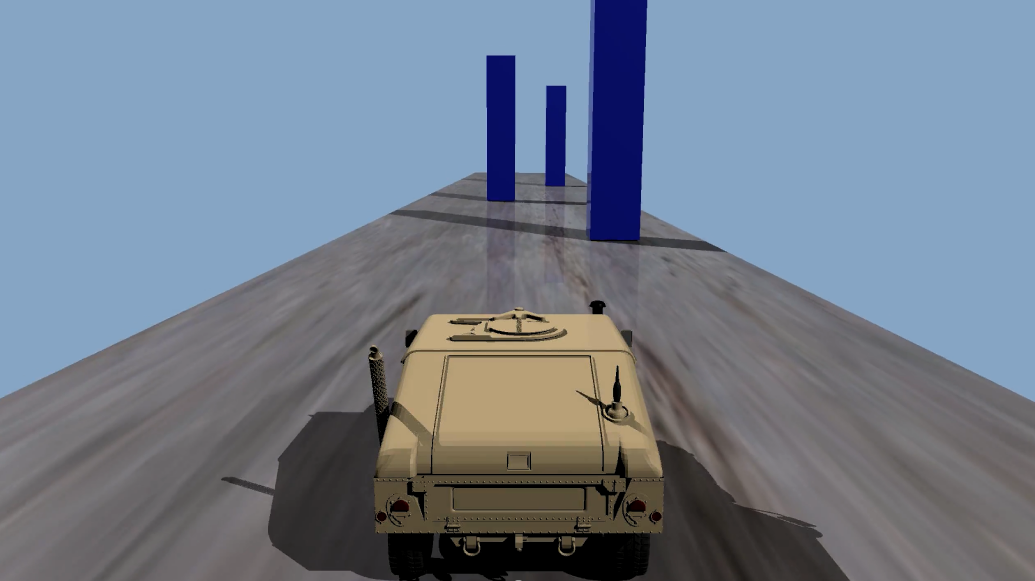
\includegraphics[width=0.75\textwidth]{ProcSci_TeX/Figures/obst_aovid.png}
    \caption{Obstacle Avoidance Environment}
    \label{fig:Obst_avoid}
 \end{minipage}
\end{figure}

\subsubsection{Autonomous Driving Environments}
These environments leverage the \textit{vehicle} and \textit{sensor} modules to reproduce autonomous driving scenarios, and are divided into 2 sub-categories:
\begin{itemize}
    \item Vision-only: \newline
    These environments observation is an RGB image, thus the cannot navigate if the direction is not encoded in the image (such as in the cone track). We provide an obstacle avoidance (figure\ref{fig:Obst_avoid}) and a cone-track environment (figure \ref{fig:Hallway})
    \item Sensor Fusion: \newline
    These environments observation is a set (tuple) of heterogeneous tensors, usually an image and a vector. Being able to encode the scene and the GPS information in the state they are capable of autonomous navigation. This family is composed of a convoy following and a off-road navigation environments.
\end{itemize}
\section{DRL algorithm implementation}
\subsection{PPO Algorithm}
To solve this environment we wrote a custom PyTorch \cite{paszke2017PyTorch} implementation of the Clipped Objective version of the Proximal Policy optimization algorithm \cite{Schulman2017PPO}.

Let the ratio $r_t(\theta) = \frac{\pi_\theta(a_t|s_t)}{\pi_{\theta_k}(a_t|s_t)} $. Then:
\begin{equation} \label{eq:PPO_clip}
    \mathcal{L}_{\theta k}^{CLIP}(\theta) = \underset{\tau\sim\pi_k}{E}\left[\sum_{t=0}^\infty\left[\min\left(r_t(\theta)\hat{A}_t^{\pi_k}, clip\left(r_t(\theta), 1-\epsilon, 1+\epsilon\right)\right)\hat{A}_t^{\pi_k}\right]\right] 
\end{equation}
With:
\begin{itemize}
    \item[$t$]{timestep. The sum to $\infty$ is a generalization, in finite horizon scenarios the sum ends a t the terminal step. The data might be collected over multiple simulation, in this case in the sum there will be several initial and terminal timesteps.}
    \item[$a_t$]{Action at timestep t}
    \item[$s_t$]{State at timestep t}
    \item[$\theta$]{Policy NN parameters}
    \item[$\pi_\theta$]{Policy, the probability distribution of actions given the state. $\pi_\theta(a_t|s_t)$ is the probability of taking the action $a_t$ in state $s_t$}
    \item[$\epsilon$]{Clipping ratio, $\sim 0.2$}
    \item[$k$]{The k-th parameter update. Before the update the parameters are $\theta_k$, and the Advantage Function is estimated on the Policy $\pi_{\theta_k}$}.
    \item[$\hat{A}_t^{\pi_k}$]{Estimate of the Advantage Function at timestep t w.r.t. the policy $\pi_{\theta_k}$}
\end{itemize}
We mentioned the Advantage Function. To define it, we first need to introduce the \textit{State Value Function} (or often only Value Function, also VF) as:
\begin{equation} \label{eq:stateVF}
    V^\pi(s_t) \quad := \quad \mathbb{ E} \left[ \sum_{l=0}^\infty \gamma^l r_{t+l} \;|\; s_t \right] 
\end{equation}
Where:
\begin{itemize}
    \item $r:{t+l}$ is the Reward at timestep $t+l$
    \item $\gamma$ is the discount factor
\end{itemize}
The VF, being the expected value of the (disconuted) sum of future reward given the current policy $\pi$, tells how much a state is \textit{good} when following the current policy.

The Advantege Function (AF) is defined as:
%\begin{equation} \label{eq:AdfFunct}
%    A^\pi(s_t, a_t) := r_t + \gamma V^\pi(s_{t+1}) - V^\pi(s_t)
%\end{equation}
\begin{equation}\label{eq:TDeq} A^{\pi,\gamma} = \mathbb{E}_{s^{t+1}}\left[r_t+\gamma V^{\pi,\gamma}(s_{t+1})- V^{\pi,\gamma}(s_t)\right] = E_{s^{t+1}}\left[\delta_t^{V^{\pi,\gamma}}\right]
\end{equation}
Being affected by a lower variance, it is more convenient to estimate the VF through a NN rather than the AF, using the unbiased estimator proposed by Schulman et al. \cite{Schulman15GAE}.

The generalized advantage estimator GAE($\gamma, \lambda)$ is defined as a $\lambda$ exponentially-weighted average:
\begin{equation}\label{eq:GAE}
\hat{A}_t^{GAE(\gamma,\lambda)} = \sum_{l=0}^\infty(\gamma\lambda)^l\delta_{t+l}^V
\end{equation}


\subsection{Continuous Control}
When using a DRL technique with a stochastic policy we must sample the action from a distribution determined by the NN. To do so, in continuous task, the typical solution is to sample the action from a multivariate gaussian distribution. The means of the distributions are the NN outputs, while the variances are an optimizable parameters. Variances are high during the early stages of the training to encourage exploration and narrows down as the policy converges.
%\begin{figure}[ht]
%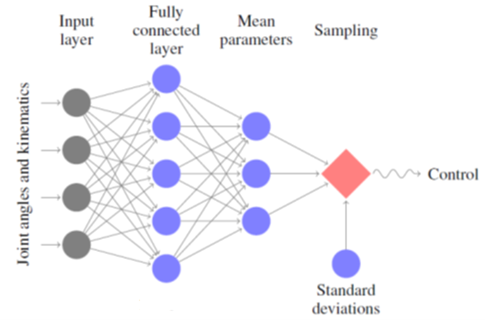
\includegraphics[width=0.75\textwidth]{ProcSci_TeX/Figures/action_sampling.png}
%\caption{Action sampling from a NN output.}
%\label{fig:act_sampl}
%\end{figure}

%\subsection{NN architectures}

\subsubsection{Implementation Details and Features}
Our custom implementation of the PPO algorithm relies on PyTorch DL framework and uses Adam optimizer

Our algorithm is able to deal with vector, image and image+vector tuple inputs, given that the right NN model is called (we also provide several NN architecture to accommodate different input shapes).

\section{Results obtained}
Using the aforementioned algorithm, with different NN architecture according to the observation shape, we have been able to train the autonomous agents to solve all the task of gym-chrono, while we mention here just a couple of them for sake of brevity.

\paragraph{Hexapod}
The Hexapod walker is the gym-chrono environment featuring the highest number of actions, thus being the hardest of robotics environments. In fact, as reported in figure \ref{fig:Hexa_rew}, it took 6000 episodes to converge, being almost 3 times the number of policy updates required by the robotic arm.

\begin{figure}[ht]
 \begin{minipage}[b]{0.6\linewidth}
    \centering
    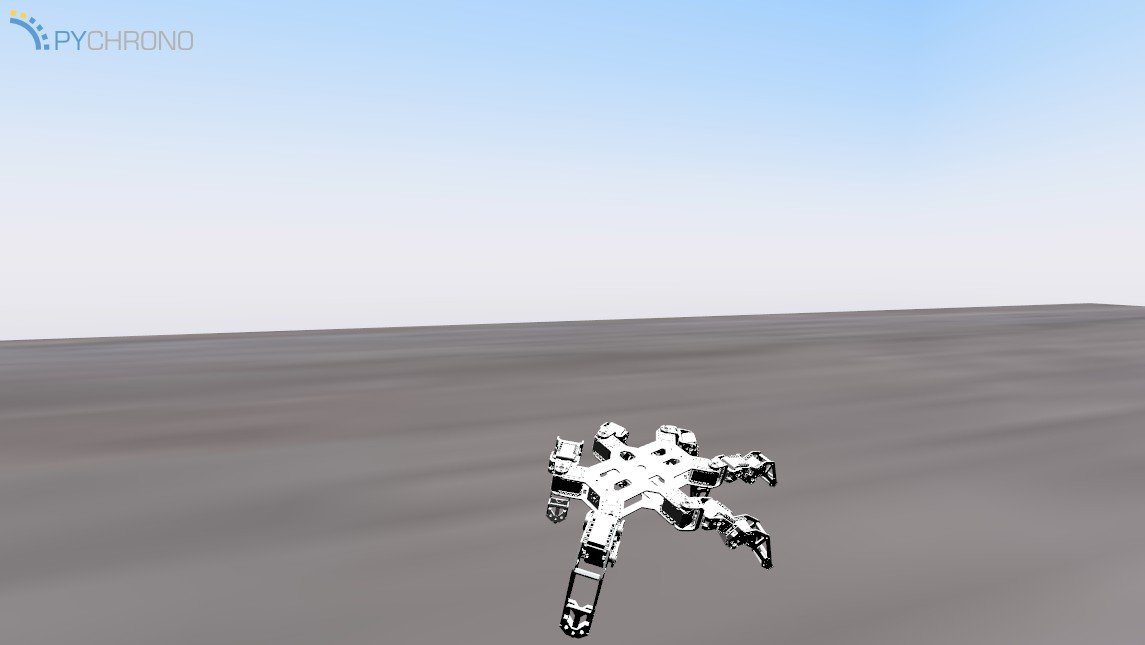
\includegraphics[width=0.75\textwidth]{ProcSci_TeX/Figures/Hexapod.jpg}
    \caption{Hexapod Environment}
    \label{fig:Hexa}
 \end{minipage}
 %\hspace{0.4cm}
 \begin{minipage}[b]{0.6\linewidth}
    \centering
    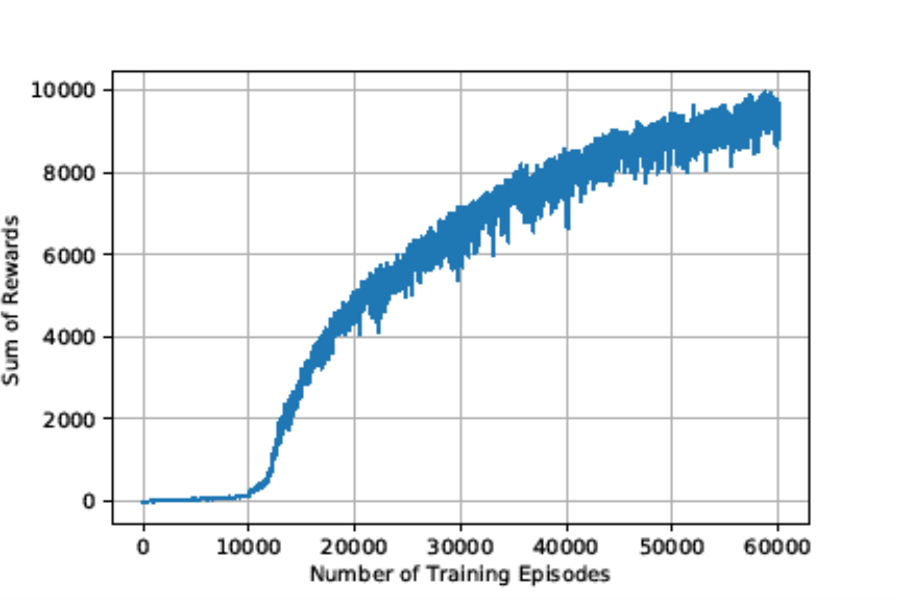
\includegraphics[width=0.75\textwidth]{ProcSci_TeX/Figures/hexa_rew.png}
    \caption{Hexapod Reward Progression}
    \label{fig:Hexa_rew}
 \end{minipage}
\end{figure}

\paragraph{Hallway cone track}
In this environment \ref{fig:Hallway} a model of a RC car has to drive in a reproduction of a real indoor hallway in a track delimited by red and green cones. The agent only controls 1 action (the steering) since the speed is feed-back controlled to keep a constant value, thus the convergence can be reached in a relatively short amount of iteration (as shown in figure \ref{fig:Hallway_rew}). This being said, this scenario proves the capability of PyChrono of dealing with large scenarios (the hallway 3D mesh) and large dataset (the 160x90 image observation is the largest of the set). In addition, this environment could be solved only after the starting position was placed in proximity of a turn. Starting on a straight, with a 0 steering angle, means starting in a local maximum that the algorithm is likely to overfit. 

\begin{figure}[ht]
 \begin{minipage}[b]{0.6\linewidth}
    \centering
    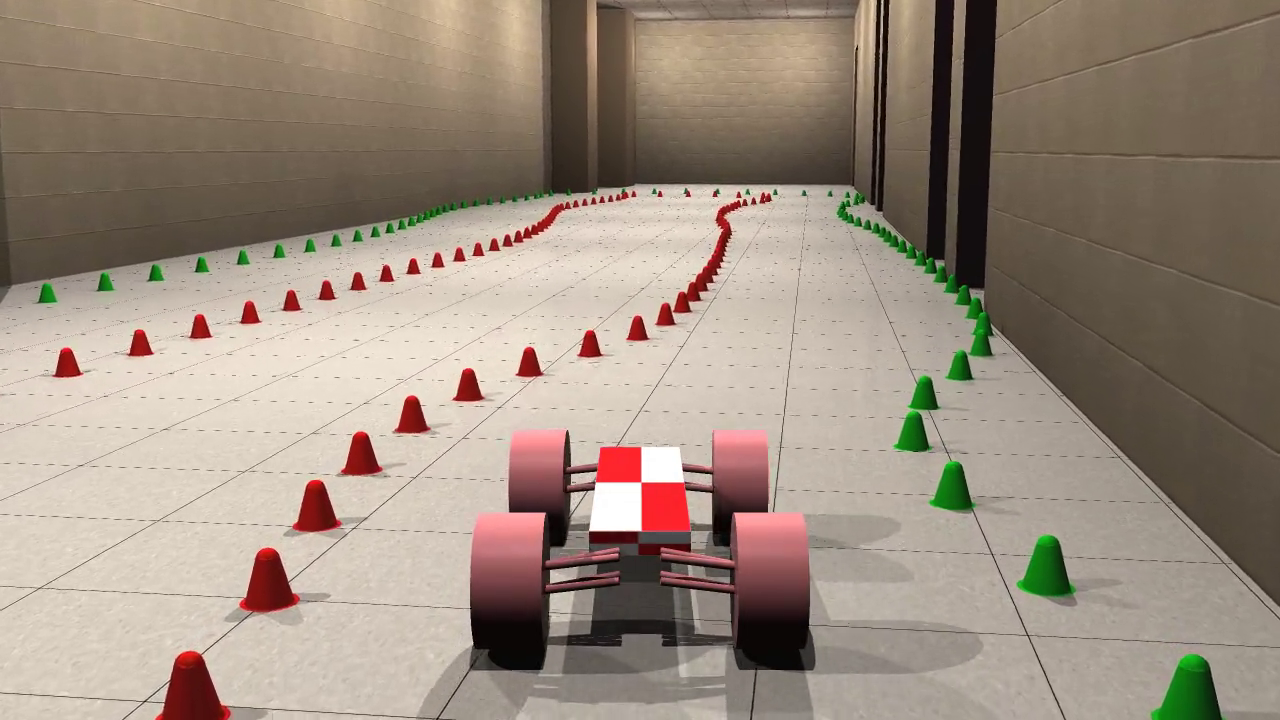
\includegraphics[width=0.75\textwidth]{ProcSci_TeX/Figures/hallway.png}
    \caption{Hallway Cone Track Environment}
    \label{fig:Hallway}
 \end{minipage}
 %\hspace{0.4cm}
 \begin{minipage}[b]{0.6\linewidth}
    \centering
    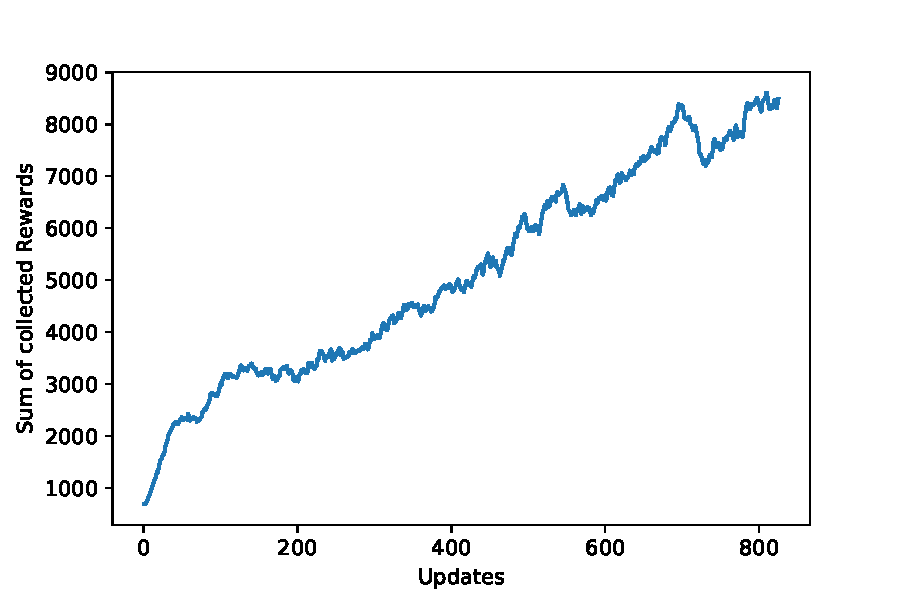
\includegraphics[width=0.75\textwidth]{ProcSci_TeX/Figures/hallway_rewards.pdf}
    \caption{Hallway Cone Track Reward Progression}
    \label{fig:Hallway_rew}
 \end{minipage}
\end{figure}


\section{Conclusions}
%containing the core  findings and highlights  of the work. 
Together with a a concerted effort to improve the Python wrappers of Chrono, that lead to an Anaconda-distributed package with a good user base \cite{pyChronoCondaWebSite}, we built a set of increasingly challenging DRL environments, and used state-of-the-art continuous actions DRL algorithms to solve them. The first step has been building and solving environments such as the inverted pendulum and the 4-legged walker \cite{Benatti194Legs}. Then, we included models of real 6-DOF robots by leveraging the tools for 3D CAD parsing of Chrono \cite{Benatti19Solidworks}, and more complex, real-world robotic walkers. This feature proved to be useful by making changes in the model extremely easy to be passed to the training environment.

The latest development have been in the field of autonomous driving in off-road conditions, simulating vehicle dynamics and terrain deformation. In this context, we have been able to train autonomous agents to navigate in off-road unknown scenarios with obstacles and height irregularities to reach a target location.
These results have been made possible by the capabilities of Chrono in Vehicle and Sensor simulation, whose API allows to model vehicle and attach sensors to them, easing the creation of autonomous driving virtual environments, while providing detailed models of vehicles and terrain for accurate physical simulation.

\bibliographystyle{plain}
\bibliography{Bib/DRL, Bib/refsMBS, Bib/refsChronoSpecific, Bib/refsAutonomousVehicles}



\end{document}